\renewcommand{\myleftmark}{{\Large Επανάληψη Α' και Β' Λυκείου}}
\begin{center}
\part{Επανάληψη Α' και Β' Λυκείου}
\end{center}
\section{Σύνολα}
\begin{enumerate}
\item Βασικά σύνολα αριθμών
\begin{multicols}{2}
\begin{alist}[leftmargin=4mm]
\item Φυσικοί αριθμοί : $ \mathbb{N}=\{0,1,2,3,\ldots\} $.
\item Ακέραιοι αριθμοί : $ \mathbb{Z}=\{\ldots,-2,-1,0,1,2,\ldots\} $.
\item Ρητοί αριθμοί : $ \mathbb{Q}=\left\lbrace \left. \frac{a}{\beta}\right|a,\beta\in\mathbb{Z},\beta\neq0\;\right\rbrace  $.
\item Άρρητοι αριθμοί : Κάθε αριθμός που δεν είναι ρητός.
\item Πραγματικοί αριθμοί : $\mathbb{R}=\{ \textrm{όλοι οι αριθμοί} \} $.
\end{alist}
\end{multicols}
\item Πράξεις μεταξύ συνόλων
\begin{multicols}{2}
\begin{alist}
\item Ένωση : $ A\cup B=\left\lbrace x\in\varOmega\left| x\in A \textrm{ ή } x\in B\right.\right\rbrace $
\item Τομή : $ A\cap B=\left\lbrace x\in\varOmega\left| x\in A \textrm{ και } x\in B\right.\right\rbrace $
\item Συμπλήρωμα : $ A'=\left\lbrace x\in\varOmega\left| x\notin A\right.\right\rbrace $
\item Διαφορά : $ A-B=\left\lbrace x\in\varOmega\left| x\in A\textrm{ και }x\notin B\right. \right\rbrace $
\end{alist}
\end{multicols}
\end{enumerate}
\section{Πραγματικοί αριθμοί}
\paragraph{Ιδιότητες ισοτήτων}
%\begin{multicols}{2}
\begin{alist}
\begin{minipage}{0.4\linewidth}
\item $a=\beta\Leftrightarrow a+\gamma=\beta+\gamma$
\item $a=\beta\Leftrightarrow a-\gamma=\beta-\gamma$
\item $a=\beta\Leftrightarrow a\cdot\gamma=\beta\cdot\gamma$
\end{minipage}
\begin{minipage}{0.6\linewidth}
\item $a=\beta\Leftrightarrow \dfrac{a}{\gamma}=\dfrac{\beta}{\gamma}\;,\;\gamma\neq0$
\item $a=\beta\Rightarrow a^\nu=\beta^\nu$
\item $a=\beta\Leftrightarrow\sqrt[\nu]{a}=\!\sqrt[\nu]{\beta}$ όπου $ a,\beta>0 $, $ \nu\in\mathbb{N} $.
\end{minipage}
\item Πρόσθεση κατά μέλη: $a=\beta\textrm{ και }\gamma=\delta\Leftrightarrow a+\gamma=\beta+\delta$
\item Αφαίρεση κατά μέλη: $a=\beta\textrm{ και }\gamma=\delta\Leftrightarrow a-\gamma=\beta-\delta$
\item Πολλαπλασιασμός κατά μέλη: $a=\beta\textrm{ και }\gamma=\delta\Leftrightarrow a\cdot\gamma=\beta\cdot\delta$
\item Διαίρεση κατά μέλη: $a=\beta\textrm{ και }\gamma=\delta\Leftrightarrow \dfrac{a}{\gamma}=\dfrac{\beta}{\delta}\;,\;\gamma\cdot\delta\neq0$
\item $a\cdot\beta=0\Leftrightarrow a=0\textrm{ \textbf{ή} }\beta=0 $
\item $a\cdot\beta\neq0\Leftrightarrow a\neq0\textrm{ \textbf{και} }\beta\neq0$
\end{alist}
\paragraph{Ιδιότητες δυνάμεων}
Για οποιουσδήποτε πραγματικούς αριθμούς $a,\beta\in\mathbb{R}$ και φυσικούς $\nu,\mu\in\mathbb{N}$ ισχύουν οι εξής ιδιότητες:
\[ a^1=a\;\;,\;\;a^0=1\;,\;\textrm{όπου }a\neq0\;\;,\;\;a^{-\nu}=\dfrac{1}{a^\nu}\;,\;\textrm{όπου }a\neq0 \]
\begin{center}
\begin{mytblr}[long]{}
\textbf{Ιδιότητα} & \textbf{Συνθήκη} \\
Γινόμενο με κοινή βάση & $ a^\nu\cdot a^\mu=a^{\nu+\mu} $ \\
Πηλίκο με κοινή βάση & $ a^\nu: a^\mu=a^{\nu-\mu} $\\
Γινόμενο με κοινό εκθέτη & $ \left(a\cdot\beta\right)^\nu=a^\nu\cdot\beta^\nu $ \\
Πηλίκο με κοινό εκθέτη & $ \left(\dfrac{a}{\beta}\right)^\nu=\dfrac{a^\nu}{\beta^\nu}\;\;,\;\;\beta\neq0 $ \\
Δύναμη υψωμένη σε εκθέτη & $ \left( a^\nu\right)^\mu=a^{\nu\cdot\mu} $ \\
Κλάσμα με αρνητικό εκθέτη & $ \left( \dfrac{a}{\beta}\right)^{-\nu}=\left(\dfrac{\beta}{a}\right)^\nu\;\;,\;\;a,\beta\neq0 $
\end{mytblr}\captionof{table}{Ιδιότητες δυνάμεων}
\end{center}
\vspace{-5mm}
\paragraph{Βασικές ταυτότητες}
\begin{multicols}{2}
\begin{alist}[itemsep=0mm]
\item $ (a+\beta)^2=a^2+2a\beta+\beta^2 $
\item $ (a-\beta)^2=a^2-2a\beta+\beta^2 $
\item $ (a+\beta)^3=a^3+3a^2\beta+3a\beta^2+\beta^3 $
\item $ (a-\beta)^3=a^3-3a^2\beta+3a\beta^2-\beta^3 $
\item $ (a+\beta)(a-\beta)=a^2-\beta^2 $
\item$ (a+\beta)\left(a^2-a\beta+\beta^2 \right)=a^3+\beta^3 $
\item $ (a-\beta)\left(a^2+a\beta+\beta^2 \right)=a^3-\beta^3 $
\end{alist}
\end{multicols}
\paragraph{Βασικοί τρόποι παραγοντοποίησης}
\begin{enumerate}
\item Κοινός παράγοντας: $a\cdot\beta+a\cdot\gamma=a\cdot(\beta+\gamma)$.
\begin{itemize}
\item Από τους συντελεστές των όρων, βγάζουμε κοινό παράγοντα το Μ.Κ.Δ. τους.
\item Από τους άγνωστους παράγοντες, βγάζουμε τις κοινές μεταβλητές ή παραστάσεις, υψωμένες στο μικρότερο εκθέτη.
\item Διαιρούμε κάθε όρο με τον κοινό παράγοντα ώστε να βρούμε τος όρους που θα μπουν στην παρένθεση.
\end{itemize}
\item Ομαδοποίηση:
\item Διαφορά τετραγώνων:
\item Διαφορά κύβων:
\item Άθροισμα κύβων:
\item Ανάπτυγμα τετραγώνου:
\item Τριώνυμο $ax^2+\beta x+\gamma$:\\
\begin{mytblr}{}
\textbf{Διακρίνουσα - Ρίζες} & \textbf{Παραγοντοποίηση}\\
$\varDelta>0$: 2 ρίζες $x_1,x_2$ & $ax^2+\beta x+\gamma=a(x-x_1)(x-x_2)$\\
$\varDelta>0$: 1 ρίζα $x_0$ & $ax^2+\beta x+\gamma=a(x-x_0)^2$\\
$\varDelta>0$: Καμία ρίζα & Δεν παραγοντοποιείται
\end{mytblr}
\item Τέλεια διαίρεση - σχήμα \eng Horner\gr:
\end{enumerate}
\Paradeigma{Παραγοντοποίηση}
\bmath{}\\
\lysh
\begin{alist}
\item 
\end{alist}
\paragraph{Ιδιότητες διάταξης}
\begin{alist}
\begin{multicols}{2}
\item Αν $ a>\beta $ και $ \beta>\gamma \Rightarrow a>\gamma $.
\item 
\begin{itemize}
\item Αν $ a>0 $ και $ \beta>0 $ τότε $ a+\beta>0 $.
\item Αν $ a<0 $ και $ \beta<0 $ τότε $ a+\beta<0 $.
\end{itemize}
\item Αν $ a,\beta\ \textrm{ομόσημοι}\ \Leftrightarrow a\cdot\beta>0\ \textrm{και}\ \frac{a}{\beta}>0 $.
\item Αν $ a,\beta\ \textrm{ετερόσημοι}\ \Leftrightarrow a\cdot\beta<0\ \textrm{και}\ \frac{a}{\beta}<0 $.
\item Αν $ a>\beta\Leftrightarrow a+\gamma>\beta+\gamma\ \textrm{και}\ a-\gamma>\beta-\gamma $.
\end{multicols}
\item 
\begin{itemize}
\item $ \textrm{Αν }\gamma>0\textrm{ τότε }a>\beta\Leftrightarrow a\cdot\gamma>\beta\cdot\gamma\textrm{ και }\dfrac{a}{\gamma}>\dfrac{\beta}{\gamma} $
\item $ \textrm{Αν }\gamma<0\textrm{ τότε }a>\beta\Leftrightarrow a\cdot\gamma<\beta\cdot\gamma\textrm{ και }\dfrac{a}{\gamma}<\dfrac{\beta}{\gamma} $
\end{itemize}
\item $ \textrm{Αν }a,\beta\textrm{ ομόσημοι τότε } a>\beta\Leftrightarrow \dfrac{1}{a}<\dfrac{1}{\beta} $
\item Πρόσθεση κατά μέλη  $a>\beta\;\;\textrm{και}\;\;\gamma>\delta\Leftrightarrow a+\gamma>\beta+\delta$
\item Πολλαπλασιασμός κατά μέλη
 $a>\beta\;\;\textrm{και}\;\;\gamma>\delta\Leftrightarrow a\cdot\gamma>\beta\cdot\delta\;\;,\;\;\textrm{με }a,\beta,\gamma,\delta>0$
\item \textbf{Δεν} μπορούμε να αφαιρέσουμε ή να διαιρέσουμε ανισότητες κατά μέλη.
\end{alist}
...Δύναμη με άρτιο εκθέτη : $a^2\geq0\ \ ,\ \ a^{2\kappa}\geq0\;\;,\;\;\kappa\in\mathbb{Z}$
\paragraph{Απολυτή τιμή πραγματικού αριθμού}
\begin{center}
\begin{tabular}{c >{\centering\arraybackslash}m{6cm}}
$ |a|=\begin{cases}
\begin{aligned}
a & \;,\;a\geq0\\
-a & \;,\;a<0
\end{aligned}
\end{cases} $  & 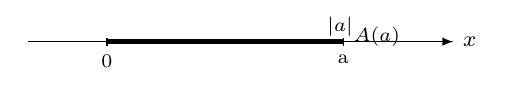
\begin{tikzpicture}
\draw[-latex] (-1,0) -- coordinate (x axis mid) (4.4,0) node[right,fill=white] {{\footnotesize $ x $}};
\draw (0,.5mm) -- (0,-.5mm) node[anchor=north,fill=white] {{\scriptsize 0}};
\draw (3,.5mm) -- (3,-.5mm) node[anchor=north,fill=white] {{\scriptsize a}};
\draw[line width=.7mm] (0,0) -- (3,0);
\tkzText(1.5,.34){$ \overcbrace{\rule{28mm}{0mm}}^{{\scriptsize |a|}} $}
\tkzDefPoint(3,0){A}
\tkzDrawPoint[size=3,fill=white](A)
\tkzLabelPoint[above right](A){{\scriptsize $A(a)$}}
\end{tikzpicture}
\end{tabular} 
\end{center}
.............
\[ |a-\beta|=d(a,\beta) \]
Ιδιότητες απόλυτων τιμών
\begin{center}
\begin{mytblr}{}
\textbf{Ιδιότητα} & \textbf{Συνθήκη} \\
Πρόσημο απόλυτης τιμής & $ |a|=|-a|\geq0 $ \\
Απόλυτη τιμή μηδενός & $ |a|=0\Leftrightarrow a=0 $\\
Σχέση μεταξύ $a$ και $|a|$ & $ -|a|\leq a\leq|a| $ \\
Απόλυτη τιμή γινομένου & $ |a\cdot\beta|=|a|\cdot|\beta| $ \\
Απόλυτη τιμή πηλίκου & $ \left| \dfrac{a}{\beta}\right|=\dfrac{|a|}{|\beta|} $ \\
Τετράγωνο απόλυτης τιμής & $ |a|^2=a^2 $ \\
Τριγωνική ανισότητα & $ \left||a-\beta| \right|\leq|a\pm\beta|\leq|a|+|\beta|  $
\end{mytblr}\captionof{figure}{Ιδιότητες απόλυτων τιμών}
\end{center}
\paragraph{Τετραγωνική ρίζα - Ρίζα \MakeLowercase{ν}-τάξης}
$ \sqrt{x}=a\;\;,\;\;\textrm{ όπου }x\geq0\textrm{ και }a\geq0 $
\begin{itemize}[itemsep=0mm]
\item Ο αριθμός $ x $ ονομάζεται \textbf{υπόριζο}.
\item Δεν ορίζεται ρίζα αρνητικού αριθμού.
\end{itemize}
$ \sqrt[\nu]{x}=a\;\;,\;\;\textrm{ όπου }x\geq0\textrm{ και }a\geq0 $.
Δύναμη με ρητό εκθέτη : $ a^{\frac{\mu}{\nu}}=\!\sqrt[\nu]{a^\mu}\ ,\ \textrm{ όπου } a>0  $\\
{Ιδιότητες Ριζών}
\begin{center}
\begin{mytblr}[long]{}
\textbf{Ιδιότητα} & \textbf{Συνθήκη} \\
Τετράγωνο ρίζας & $ \left(\!\sqrt{x}\;\right)^2=x\;\;,\;\; x\geq0  $ \\
Ν-οστή δύναμη ν-οστής ρίζας & $ \left(\!\sqrt[\nu]{x}\;\right)^\nu=x\;\;,\;\; x\geq0  $ \\
Ρίζα τετραγώνου & $ \sqrt{x^2}=|x|\;\;,\;\; x\in\mathbb{R} $\\
Ν-οστή ρίζα ν-οστής δύναμης & $ \sqrt[\nu]{x^\nu}=\begin{cases}
|x|&  x\in\mathbb{R}\textrm{ αν }\nu\textrm{ άρτιος}\\x&  x\geq0\textrm{ και } \nu\in\mathbb{N}\end{cases} $\\
\SetCell[r=2]{m} Ρίζα γινομένου & $ \sqrt{x\cdot y}=\!\sqrt{x}\cdot\!\sqrt{y}\;\;,\;\; x,y\geq0 $ \\
& $ \sqrt[\nu]{x\cdot y}=\!\sqrt[\nu]{x}\cdot\!\sqrt[\nu]{y}\;\;,\;\; x,y\geq0 $ \\
\SetCell[r=2]{m,bg=red9} Ρίζα πηλίκου & $ \sqrt{\dfrac{x}{y}}\;=\dfrac{\sqrt{x}}{\sqrt{y}}\;\;,\;\; x\geq0\textrm{ και }y>0 $ \\
& $ \sqrt[\nu]{\dfrac{x}{y}}\;=\dfrac{\sqrt[\nu]{x}}{\sqrt[\nu]{y}}\;\;,\;\; x\geq0\textrm{ και }y>0 $ \\
Απλοποίηση ρίζας & $ \sqrt[\nu]{x^\nu\cdot y}=x\!\sqrt[\nu]{y}\;\;,\;\; x,y\geq0  $
\end{mytblr}\captionof{table}{Ιδιότητες ριζών}
\end{center}
\section{Εξισώσεις}
\paragraph{Εξισώσεις 1\tssL{ου} βαθμού} $ax+\beta=0$ όπου $ a,\beta\in\mathbb{R} $ και λύσεις:
\begin{center}
\begin{mytblr}{}
\SetCell[c=2]{c} Συντελεστές & & Λύσεις \\ 
\SetCell[c=2]{c} $a\neq0$ & & $ x=-\frac{\beta}{a} $ μοναδική λύση\\ 
\SetCell[r=2]{c}$a=0$ & $ \beta=0 $ & $ 0x=0 $ αόριστη - άπειρες λύσεις \\
& $ \beta\neq0 $ & $ 0x=\beta $ αδύνατη - καμία λύση 
\end{mytblr}\captionof{table}{Λύσεις εξίσωσης 1\textsuperscript{ου} βαθμού}
\end{center}
\begin{multicols}{2}
\paragraph{Εξισώσεις με απόλυτες τιμές}
\begin{itemize}[itemsep=0mm]
\item Η εξίσωση $ |x|=a $ :
\begin{alist}[itemsep=0mm]
\item Αν $ a>0 $ τότε : $ |x|=a\Leftrightarrow x=\pm a $
\item Αν $ a=0 $ τότε : $ |x|=0\Leftrightarrow x=0 $
\item Αν $ a<0 $ τότε η εξίσωση είναι αδύνατη.
\end{alist}
\item $ |x|=|a|\Leftrightarrow x=\pm a $
\end{itemize}
\vspace{3mm}
\paragraph{Εξισώσεις της μορφής \MakeLowercase{\bmath{$x^\nu=a $}}}
\begin{mytblr}{}
& $a>0$ & $a<0$\\ 
$\nu$ άρτιος & $ x=\pm\sqrt[\nu]{a} $ & Αδύνατη \\
$\nu$ περιττός & $x=\sqrt[\nu]{a}$ & $x=-\sqrt[\nu]{|a|}$
\end{mytblr}\captionof{table}{Λύσεις εξίσωσης $x^{\nu}=a$}
\end{multicols}
\paragraph{Εξισώσεις 2\tssL{ου} βαθμού}
$ ax^2+\beta x+\gamma=0\;\;,\;\;a\neq0 $ και λύσεις
\begin{center}
\begin{mytblr}{}
Διακρίνουσα & Πλήθος λύσεων & Λύσεις \\ 
$ \varDelta>0 $ &  2 πραγματικές άνισες λύσεις & $ x_{1,2}=\dfrac{-\beta\pm\!\sqrt{\varDelta}}{2a} $  \\
$ \varDelta=0 $ & 1 διπλή πραγματική λύση & $ x=-\dfrac{\beta}{2a} $\\
$ \varDelta<0 $ & \SetCell[c=2]{c} Καμία πραγματική λύση - Αδύνατη στο $ \mathbb{R} $ 
\end{mytblr}\captionof{table}{Λύσεις εξίσωσης 2\tss{ου} βαθμού}
\end{center}
\paragraph{Εξισώσεις 3\tssL{ου+} βαθμού}
\paragraph{Κλασματικές ανισώσεις}
\paragraph{Άρρητες ανισώσεις}
\section{Ανισώσεις}
\paragraph{Ανισώσεις 1\tss{ου} βαθμού} $ax+\beta>0$ ή $ax+\beta<0$.
\paragraph{Ανισώσεις 1\tss{ου} βαθμού}
$ ax^2+\beta x+\gamma=0\;\;,\;\;a\neq0 $
\begin{center}
\begin{tikzpicture}
\tikzset{t style/.style = {style = dashed}}
\tikzset{z style/.style = {fill=white,inner sep=.2mm}}
\tkzTabInit[color,lgt=2.7,espcl=2,colorC = red7,
colorL = red9,
colorV = red7]%
{$x$ / .8,$ax^2+\beta x+\gamma$ /1.2}%
{$-\infty$,$x_1$,$x_2$,$+\infty$}%
\tkzTabLine{ , \genfrac{}{}{0pt}{0}{\text{Ομόσημο}}{ \text{του } a}, z
, \genfrac{}{}{0pt}{0}{\text{Ετερόσημο}}{ \text{του } a}, z
, \genfrac{}{}{0pt}{0}{\text{Ομόσημο}}{ \text{του } a}, }
\end{tikzpicture}\captionof{table}{Πρόσημα τριωνύμου με $\varDelta>0$}\mbox{}\\
\begin{multicols}{2}
\begin{tikzpicture}
\tikzset{t style/.style = {style = dashed}}
\tkzTabInit[color,lgt=2.7,espcl=2,colorC = red7,
colorL = red9,
colorV = red7]%
{$x$ / .8,$ax^2+\beta x+\gamma$ /1.2}%
{$-\infty$,$x_0$,$+\infty$}%
\tkzTabLine{ , \genfrac{}{}{0pt}{0}{\text{Ομόσημο}}{ \text{του } a}, z
, \genfrac{}{}{0pt}{0}{\text{Ομόσημο}}{ \text{του } a}, }
\end{tikzpicture}\captionof{table}{Πρόσημα τριωνύμου με $\varDelta=0$}\quad
\begin{tikzpicture}
\tikzset{t style/.style = {style = dashed}}
\tkzTabInit[color,lgt=2.7,espcl=3.4,colorC = red7,
colorL = red9,
colorV = red7]%
{$x$ / .8,$ax^2+\beta x+\gamma$ /1.2}%
{$-\infty$,$+\infty$}%
\tkzTabLine{, \genfrac{}{}{0pt}{0}{\text{Ομόσημο}}{ \text{του } a}, }
\end{tikzpicture}\captionof{table}{Πρόσημα τριωνύμου με $\varDelta<0$}
\end{multicols}
\end{center}
\paragraph{Ανισώσεις με απόλυτη τιμή}
\paragraph{Κλασματικές ανισώσεις}
\section{Τριγωνομετρία}
\paragraph{Τριγωνομετρικοί αριθμοί}
\begin{center}
\begin{mytblr}{} \SetCell[c=9]{c}{\textbf{\MakeUppercase{Βασικές Γωνίες}}}\\ 
\SetRow{m}\textbf{Θέση} & \SetCell{wd=1.2cm}\textbf{Σημείο άξονα} & \SetCell[c=3]{c}{\textbf{1\tss{ο} Τεταρτημόριο}} & & & \SetCell[c=4]{c}{\textbf{Σημείο άξονα}}\\
\rule[-2ex]{0pt}{5ex} \textbf{Μοίρες} & $ 0\degree $ & $ 30\degree $ & $ 45\degree $ & $ 60\degree $ & $ 90\degree $ & $ 180\degree $ & $ 270\degree $ & $ 360\degree $ \\
\textbf{Ακτίνια} & $ 0 $ & $ \frac{\pi}{6} $ & $ \frac{\pi}{4} $ & $ \frac{\pi}{3} $ & $ \frac{\pi}{2} $ & $ \pi $ & $ \frac{3\pi}{2} $ & $ 2\pi $ \\ 
\SetCell{m}\textbf{Σχήμα} & \begin{tikzpicture}
\fill[fill=\xrwma!50] (0,0) -- (.3,0) arc (0:0:.3) -- cycle;
\draw (-.35,0) -- (.35,0);
\draw (0,-.35) -- (0,.35);
\draw (0,0) circle (.3);
\coordinate (A) at (0:.3);
\draw (0,0) -- (A);
\end{tikzpicture} & \begin{tikzpicture}
\fill[fill=\xrwma!50] (0,0) -- (.3,0) arc (0:30:.3) -- cycle;
\draw (-.35,0) -- (.35,0);
\draw (0,-.35) -- (0,.35);
\draw (0,0) circle (.3);
\coordinate (A) at (30:.3);
\draw (0,0) -- (A);
\end{tikzpicture} & \begin{tikzpicture}
\fill[fill=\xrwma!50] (0,0) -- (.3,0) arc (0:45:.3) -- cycle;
\draw (-.35,0) -- (.35,0);
\draw (0,-.35) -- (0,.35);
\draw (0,0) circle (.3);
\coordinate (A) at (45:.3);
\draw (0,0) -- (A);
\end{tikzpicture} & \begin{tikzpicture}
\fill[fill=\xrwma!50] (0,0) -- (.3,0) arc (0:60:.3) -- cycle;
\draw (-.35,0) -- (.35,0);
\draw (0,-.35) -- (0,.35);
\draw (0,0) circle (.3);
\coordinate (A) at (60:.3);
\draw (0,0) -- (A);
\end{tikzpicture} & \begin{tikzpicture}
\fill[fill=\xrwma!50] (0,0) -- (.3,0) arc (0:90:.3) -- cycle;
\draw (-.35,0) -- (.35,0);
\draw (0,-.35) -- (0,.35);
\draw (0,0) circle (.3);
\coordinate (A) at (90:.3);
\draw (0,0) -- (A);
\end{tikzpicture} & \begin{tikzpicture}
\fill[fill=\xrwma!50] (0,0) -- (.3,0) arc (0:180:.3) -- cycle;
\draw (-.35,0) -- (.35,0);
\draw (0,-.35) -- (0,.35);
\draw (0,0) circle (.3);
\end{tikzpicture} & \begin{tikzpicture}
\fill[fill=\xrwma!50] (0,0) -- (.3,0) arc (0:270:.3) -- cycle;
\draw (-.35,0) -- (.35,0);
\draw (0,-.35) -- (0,.35);
\draw (0,0) circle (.3);
\end{tikzpicture} & \begin{tikzpicture}
\fill[fill=\xrwma!50] (0,0) -- (.3,0) arc (0:360:.3) -- cycle;
\draw (-.35,0) -- (.35,0);
\draw (0,-.35) -- (0,.35);
\draw (0,0) circle (.3);
\end{tikzpicture} \\ 
$ \hm{\omega} $ & $ 0 $ & $ \frac{1}{2} $ & $ \frac{\sqrt{2}}{2} $ & $ \frac{\sqrt{3}}{2} $ & $ 1 $ & $ 0 $ & $ -1 $ & $ 0 $  \\ 
$ \syn{\omega} $ & $ 1 $ & $ \frac{\sqrt{3}}{2} $ & $ \frac{\sqrt{2}}{2} $ & $ \frac{1}{2} $ & $ 0 $ & $ -1 $ & $ 0 $ & $ 1 $  \\ 
$ \ef{\omega} $ & $ 0 $ & $ \frac{\sqrt{3}}{3} $ & $ 1 $ & $ \sqrt{3} $ & \begin{minipage}{.8cm}
\begin{center}
{\scriptsize Δεν\\\vspace{-1mm}ορίζεται}
\end{center}
\end{minipage} & $ 0 $ & 
\begin{minipage}{.8cm}
\begin{center}
{\scriptsize Δεν\\\vspace{-1mm}ορίζεται}
\end{center}
\end{minipage} & $ 0 $ \\
\rule[-2ex]{0pt}{4ex} $ \syf{\omega} $ & \begin{minipage}{.8cm}
\begin{center}
{\scriptsize Δεν\\\vspace{-1mm}ορίζεται}
\end{center}
\end{minipage} & $ \sqrt{3} $ & $ 1 $ & $ \frac{\sqrt{3}}{3} $ & $ 0 $ & \begin{minipage}{.8cm}
\begin{center}
{\scriptsize Δεν\\\vspace{-1mm}ορίζεται}
\end{center}
\end{minipage} & $ 0 $ & \begin{minipage}{.8cm}
\begin{center}
{\scriptsize Δεν\\\vspace{-1mm}ορίζεται}
\end{center}
\end{minipage} 
\end{mytblr}\captionof{table}{Τριγωνομετρικοί αριθμοί βασικών γωνιών}
\end{center}
\paragraph{Τριγωνομετρικές ταυτότητες}
\paragraph{Αναγωγή στο 1\tssL{ο} τεταρτημόριο}
\paragraph{Τριγωνομετρικές εξισώσεις}
\section{Τρίγωνα}
\section{Εξίσωση ευθείας}
\begin{enumerate}
\item Συντελεστής διεύθυνσης ευθείας: $\lambda=\ef{\omega}$ όπου $\omega$ η γωνία που σχηματίζει η ευθεία με τον άξονα $x'x$.
\item Εξίσωση ευθείας: $y=\lambda x+\beta$.
\item Αν ένα σημείο ανήκει σε μια ευθεία, τότε οι συντεταγμένες του επαληθεύουν την εξίσωσή της.
\[ M(x_0,y_0)\in(\varepsilon)\Leftrightarrow y_0=\lambda x_0+\beta \]
\item Οριζόντια ευθεία: $\varepsilon\parallel x'x\Leftrightarrow \lambda=0$.
\item Κατακόρυφη ευθεία: $\varepsilon\parallel y'y\Leftrightarrow $ δεν ορίζεται συντελεστής διεύθυνσης για την ευθεία.
\item Παράλληλες ευθείες: $\varepsilon_1\parallel\varepsilon_2\Leftrightarrow \lambda_1=\lambda_2$ αρκεί για τις ευθείες να ορίζεται συντελεστής διεύθυνσης.
\item Κάθετες ευθείες: $\varepsilon_1\perp\varepsilon_2\Leftrightarrow \lambda_1\cdot\lambda_2=-1$ αρκεί για τις ευθείες να ορίζεται συντελεστής διεύθυνσης.
\end{enumerate}